% Options for packages loaded elsewhere
\PassOptionsToPackage{unicode}{hyperref}
\PassOptionsToPackage{hyphens}{url}
%
\documentclass[
]{book}
\usepackage{lmodern}
\usepackage{amssymb,amsmath}
\usepackage{ifxetex,ifluatex}
\ifnum 0\ifxetex 1\fi\ifluatex 1\fi=0 % if pdftex
  \usepackage[T1]{fontenc}
  \usepackage[utf8]{inputenc}
  \usepackage{textcomp} % provide euro and other symbols
\else % if luatex or xetex
  \usepackage{unicode-math}
  \defaultfontfeatures{Scale=MatchLowercase}
  \defaultfontfeatures[\rmfamily]{Ligatures=TeX,Scale=1}
\fi
% Use upquote if available, for straight quotes in verbatim environments
\IfFileExists{upquote.sty}{\usepackage{upquote}}{}
\IfFileExists{microtype.sty}{% use microtype if available
  \usepackage[]{microtype}
  \UseMicrotypeSet[protrusion]{basicmath} % disable protrusion for tt fonts
}{}
\makeatletter
\@ifundefined{KOMAClassName}{% if non-KOMA class
  \IfFileExists{parskip.sty}{%
    \usepackage{parskip}
  }{% else
    \setlength{\parindent}{0pt}
    \setlength{\parskip}{6pt plus 2pt minus 1pt}}
}{% if KOMA class
  \KOMAoptions{parskip=half}}
\makeatother
\usepackage{xcolor}
\IfFileExists{xurl.sty}{\usepackage{xurl}}{} % add URL line breaks if available
\IfFileExists{bookmark.sty}{\usepackage{bookmark}}{\usepackage{hyperref}}
\hypersetup{
  pdftitle={Topology Inference for Radial Distribution Feeder based on Power Flow},
  pdfauthor={Jie Xu (s181238)},
  hidelinks,
  pdfcreator={LaTeX via pandoc}}
\urlstyle{same} % disable monospaced font for URLs
\usepackage{longtable,booktabs}
% Correct order of tables after \paragraph or \subparagraph
\usepackage{etoolbox}
\makeatletter
\patchcmd\longtable{\par}{\if@noskipsec\mbox{}\fi\par}{}{}
\makeatother
% Allow footnotes in longtable head/foot
\IfFileExists{footnotehyper.sty}{\usepackage{footnotehyper}}{\usepackage{footnote}}
\makesavenoteenv{longtable}
\usepackage{graphicx}
\makeatletter
\def\maxwidth{\ifdim\Gin@nat@width>\linewidth\linewidth\else\Gin@nat@width\fi}
\def\maxheight{\ifdim\Gin@nat@height>\textheight\textheight\else\Gin@nat@height\fi}
\makeatother
% Scale images if necessary, so that they will not overflow the page
% margins by default, and it is still possible to overwrite the defaults
% using explicit options in \includegraphics[width, height, ...]{}
\setkeys{Gin}{width=\maxwidth,height=\maxheight,keepaspectratio}
% Set default figure placement to htbp
\makeatletter
\def\fps@figure{htbp}
\makeatother
\setlength{\emergencystretch}{3em} % prevent overfull lines
\providecommand{\tightlist}{%
  \setlength{\itemsep}{0pt}\setlength{\parskip}{0pt}}
\setcounter{secnumdepth}{5}
\usepackage{booktabs}
\usepackage{amsthm}
\makeatletter
\def\thm@space@setup{%
  \thm@preskip=8pt plus 2pt minus 4pt
  \thm@postskip=\thm@preskip
}
\makeatother
\usepackage{booktabs}
\usepackage{longtable}
\usepackage{array}
\usepackage{multirow}
\usepackage{wrapfig}
\usepackage{float}
\usepackage{colortbl}
\usepackage{pdflscape}
\usepackage{tabu}
\usepackage{threeparttable}
\usepackage{threeparttablex}
\usepackage[normalem]{ulem}
\usepackage{makecell}
\usepackage{xcolor}
\usepackage[]{natbib}
\bibliographystyle{apalike}

\title{Topology Inference for Radial Distribution Feeder based on Power Flow}
\author{Jie Xu (s181238)}
\date{2020-12-12}

\begin{document}
\maketitle

{
\setcounter{tocdepth}{1}
\tableofcontents
}
\hypertarget{introduction}{%
\chapter{Introduction}\label{introduction}}

This website hosts slides for defence of my master graduation project in the
Department of Electrical Engineering at Technical University of Denmark. How
households are connected to distribution network is always unknown. A framework
to infer such connections by utilising all kinds of information is proposed in
this project.

\begin{center}\rule{0.5\linewidth}{0.5pt}\end{center}

A simple flowchart for the project is:

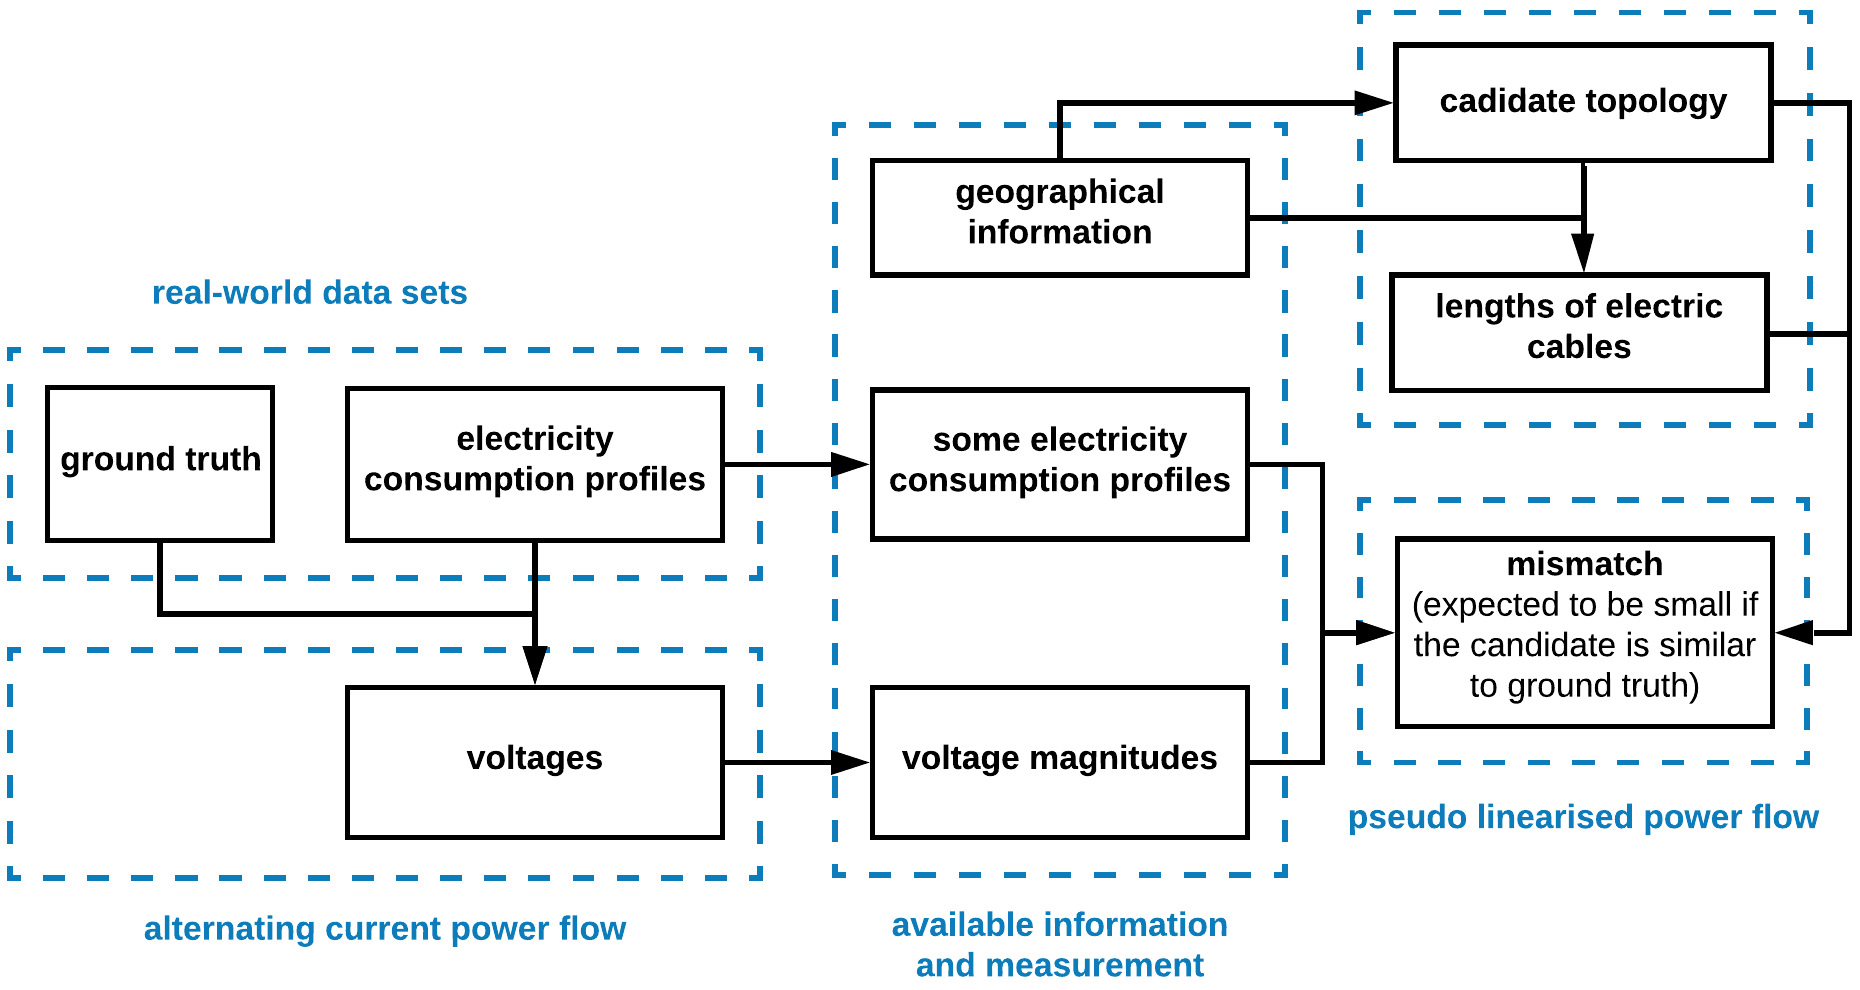
\includegraphics{Pictures/figFlowchartSimple.png}

Available information and measurement:

\begin{itemize}
\tightlist
\item
  geographical information about buses
\item
  voltage magnitudes of all the phases of all the buses
\item
  some real power injection profiles
\end{itemize}

Two batches of computer programs:

\begin{itemize}
\tightlist
\item
  alternating current power flow calculation its linearised version
\item
  three algorithms to handle directed graphs
\end{itemize}

\hypertarget{radial-distribution-feeder}{%
\chapter{Radial Distribution Feeder}\label{radial-distribution-feeder}}

\begin{itemize}
\tightlist
\item
  bus and edge
\item
  two special concepts for power flow
\item
  case with 70 buses
\end{itemize}

\hypertarget{bus-edge}{%
\section{Bus and Edge}\label{bus-edge}}

There are roughly two types of electrical devices in power grids.

\begin{table}[H]
\centering
\begin{tabular}[t]{l|l|l}
\hline
type & definition & examples\\
\hline
delivery element & transport power from one place to another & cable, transformer, capacitor\\
\hline
conversion element & convert power from or to another form & solar panel, battery\\
\hline
\end{tabular}
\end{table}

\begin{itemize}
\tightlist
\item
  Ignore conversion elements. Not necessary in power flow calculation.
\item
  Delivery element will be called \textbf{edge}.
\end{itemize}

Another concept, \textbf{bus}, represent the place where two different delivery
elements joint or end of a delivery element, but there is no physical entity
corresponding to a bus. There are three common types of buses:

\begin{table}[H]
\centering
\begin{tabular}[t]{l|l}
\hline
type & know quantities\\
\hline
slack bus & voltage magnitude and phase angle\\
\hline
PQ bus & real power injection and reactive power injection\\
\hline
PV bus & real power injection and voltage magnitude\\
\hline
\end{tabular}
\end{table}

It is sufficient to model most of RDFs with PQ buses and one kind of edges,
cables:

\begin{itemize}
\tightlist
\item
  One slack bus in RDF, corresponding to the \textbf{root}.
\item
  Root not in any matrix.
\item
  Ignore other delivery elements.
\end{itemize}

\hypertarget{two-special-concepts}{%
\section{Two Special Concepts}\label{two-special-concepts}}

Essential for power flow calculation.

\hypertarget{channel}{%
\subsection*{Channel}\label{channel}}
\addcontentsline{toc}{subsection}{Channel}

\begin{itemize}
\tightlist
\item
  \textbf{channel}: refer to one phase in some bus
\item
  \textbf{active channel}: there are non-zero injections (some conversion element is
  connected in this channel)
\item
  \textbf{observed active channel}: such non-zero injections are known
\end{itemize}

It is assumed that all active channels are known.

\hypertarget{snapshot}{%
\subsection*{Snapshot}\label{snapshot}}
\addcontentsline{toc}{subsection}{Snapshot}

\textbf{Snapshot} is a concept to include power injections and voltages at one time
index

\begin{itemize}
\tightlist
\item
  input: real power injections at all channels of PQ buses
\item
  output: voltages, current flow, power flow
\item
  Duration is 1 s in this project.
\end{itemize}

\textbf{Zero‐load snapshot} is the snapshot where power injections at all the
channels are zero and voltages equalt o rated voltages in corresponding phases.

\begin{itemize}
\tightlist
\item
  \(\boldsymbol{\bar{V}}_\text{zero}\): voltages in zero‐load snapshot
\end{itemize}

\hypertarget{case}{%
\section{Case with 70 Buses}\label{case}}

Assumptions about feeders:

\begin{itemize}
\tightlist
\item
  spanning arborescence
\item
  step-down transformer is not considered
\item
  three-phase four-wire cable
\item
  one phase star connection
\end{itemize}

\begin{center}\rule{0.5\linewidth}{0.5pt}\end{center}

A case with 70 buses is primarily used here:

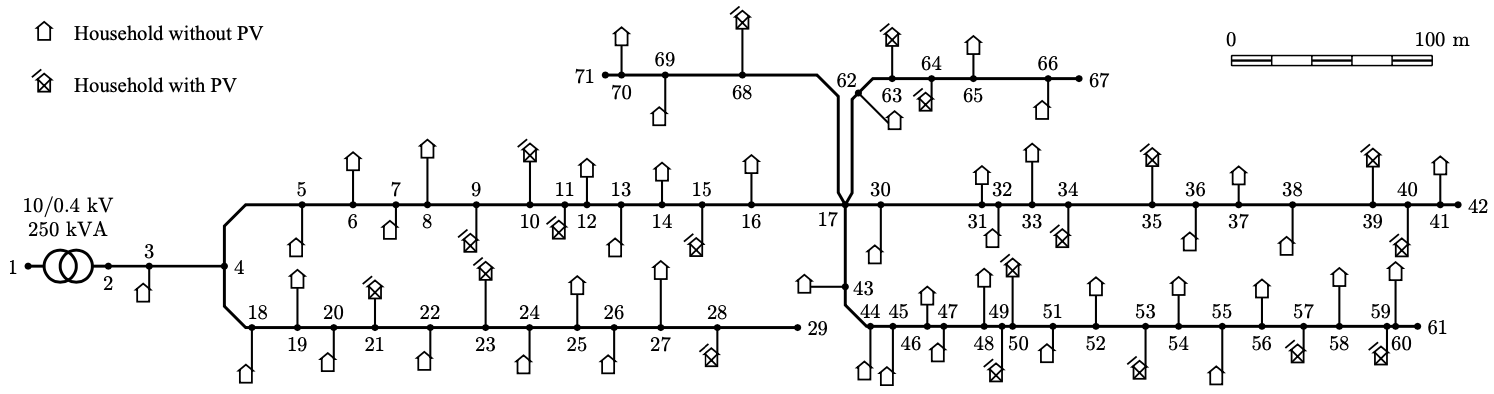
\includegraphics{Pictures/case70true.png}

\begin{itemize}
\tightlist
\item
  located in Belgium
\item
  bus 1 is omitted
\item
  Houses associated with buses 3, 7, 10, 13, 16, 20, 23, 26, 30, 33, 36, 39,
  43, 46, 49, 52, 55, 58, 62, 65, 69 are connected through phase A.
\item
  Houses associated with buses 5, 8, 11, 14, 18, 21, 24, 27, 31, 34, 37, 40,
  44, 47, 50, 53, 56, 59, 63, 66, 70 are connected through phase B.
\end{itemize}

\hypertarget{problem-formulation}{%
\chapter{Problem Formulation}\label{problem-formulation}}

\hypertarget{directed-graph}{%
\section{Directed Graph}\label{directed-graph}}

\textbf{weighted directed graph}
\(G = (\mathcal{N}, \mathcal{E}, \sigma, \tau, \omega)\)

\begin{itemize}
\tightlist
\item
  set of nodes: \(\mathcal{N}\)
\item
  set of edges: \(\mathcal{E}\)
\item
  incidence functions: source \(\sigma\), target \(\tau\)
\item
  (edge) weighting function, \(\omega: E \rightarrow \mathbb{R}\).
\item
  2-D Euclidean distance as weight
\item
  \emph{association network inference cannot be used}
\end{itemize}

\textbf{complete graph for a set of nodes}

\begin{itemize}
\tightlist
\item
  all edges are \textbf{potential edges}
\item
  some are impossible to exist
\end{itemize}

\textbf{spanning arborescence}

\begin{itemize}
\tightlist
\item
  subgraph of a directed graph
\item
  root
\item
  include every node (bus, in our case)
\end{itemize}

\textbf{feasible region}

\begin{itemize}
\tightlist
\item
  Composed of all the spanning arborescences of the directed graph.
\item
  Number of spanning arborescences is finite, making it a \protect\hyperlink{combinatorial}{combinatorial
  optimisation problem}.
\item
  To count number of spanning arborescences.
\end{itemize}

\hypertarget{overlapping}{%
\section{Remove Overlapping Edge}\label{overlapping}}

For example, in case-70:

\[
\begin{array}{lllll}
  \hline
  \textbf{shortest path} & <
  & \textbf{direct edge} & \times \textbf{threshold}
  & \text{-> } \textbf{remove direct edge} \\
  \hline
  \text{"b17‐b43-b29"} & < & \text{"b17-b29"} & \times 1.1
  & \text{-> remove "b17-b29"} \\
  \text{"b44‐b43-b29"} & > & \text{"b44-b29"} & \times 1.1
  & \text{-> keep "b44-b29"} \\
  \hline
\end{array}
\]

\begin{center}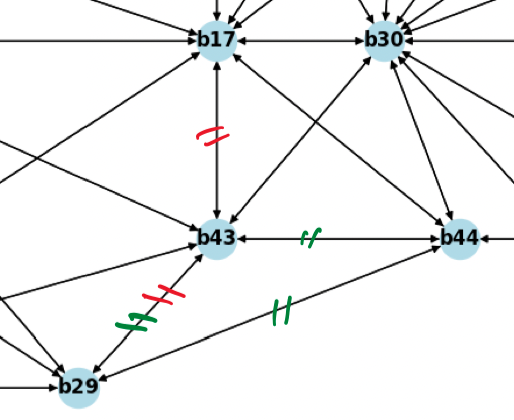
\includegraphics[width=0.7\linewidth]{Pictures/overlapGeth} \end{center}

However:

\begin{itemize}
\tightlist
\item
  446 possible potential edges
\item
  over 1045 spanning arborescences
\end{itemize}

\hypertarget{ip-formulation}{%
\section{IP Formulation}\label{ip-formulation}}

Symbols and definitions of sets:

\[
\begin{array}{ll}
  \hline
  \textbf{symbol} & \textbf{definition} \\
  \hline
  \mathcal{E}
  & \text{all the potential edges (edges in the complete graph)} \\
  \mathcal{C}
  & \text{available measurements of voltages and power injections} \\
  \mathcal{E}_\text{impossible}
  & \text{potential edges that are impossible to exist} \\
  \hline
\end{array}
\]

Symbols, definitions, types and sets of variables:

\[
\begin{array}{llll}
  \hline
  \textbf{symbol} & \textbf{definition} & \textbf{type} & \textbf{set} \\
  \hline
  x_{i j} & \text{if edge from i to j is in the solution}
  & \{0, 1\} & \mathcal{E} \\
  \hline
\end{array}
\]

Symbols, definitions, sets of constants:

\[
\begin{array}{lll}
  \hline
  \textbf{symbol} & \textbf{definition} & \textbf{set} \\
  \hline
  d_{i, j} & \text{Euclidean distance from i to j}
  & \mathcal{E} \\
  \hline
\end{array}
\]

The \textbf{integer programming formulation} is:

\[
\begin{aligned}
  \min_{x_{i j} \forall (i, j) \in \mathcal{E}} \quad
    & (1 - \alpha) \sum_{(i, j) \in \mathcal{E}} d_{i j} x_{i j}
    + \alpha \mathcal{H}
    \left(\{x_{i j} \forall (i, j) \in \mathcal{E} \}, \mathcal{C} \right) \\
  \text{s.t.} \quad & \sum_{(i, j) \in \delta^{-}(j)} x_{i j} = 1
    \quad \forall j \in V^{\prime}
    \quad \text{(a directed forest)} \\
  & \sum_{(i, j) \in \delta^{-}(S)} x_{i j} \geq 1
    \quad \forall S \subseteq V^{\prime},|S| \geq 2
    \quad \text{(a connected graph)} \\
  & x_{i j} = 0
    \quad \forall (i, j) \in \mathcal{E}_\text{impossible}
    \quad \text{(remove impossible potential edges)}
\end{aligned}
\]

Two terms in the objective function:

\[
\begin{array}{lll}
  \hline
  \textbf{term} & \textbf{definition} & \textbf{coefficient} \\
  \hline
  (1 - \alpha) \sum_{(i, j) \in \mathcal{E}} d_{i j} x_{i j}
  & \text{weight of candidate arborescence}
  & 1 - \alpha \\
  \alpha \mathcal{H}
  \left(\{x_{i j} \forall (i, j) \in \mathcal{E} \}, \mathcal{C} \right)
  & \text{assessment of candidate arborescence}
  & \alpha \\
  \hline
\end{array}
\]

Three sets of constraints:

\begin{itemize}
\tightlist
\item
  First two sets ensure arborescence.
\item
  Last set removes impossible potential edges.
\end{itemize}

\hypertarget{combinatorial}{%
\section{Combinatorial Optimisation}\label{combinatorial}}

At least two possible values for \(\alpha\):

\[
\begin{array}{llll}
  \hline
  \textbf{value} & \textbf{term lefted} & \textbf{to find}
  & \textbf{disadvantage} \\
  \hline
  1
  & \mathcal{H}
  \left(\{x_{i j} \forall (i, j) \in \mathcal{E} \}, \mathcal{C} \right)
  & \text{ground truth}
  & \text{NP-hard and non-linear} \\
  0
  & \sum_{(i, j) \in \mathcal{E}} d_{i j} x_{i j}
  & \text{topology with min total cable length}
  & \text{cannot find ground truth} \\
  \hline
\end{array}
\]

Such two situations can be visualised:

\begin{center}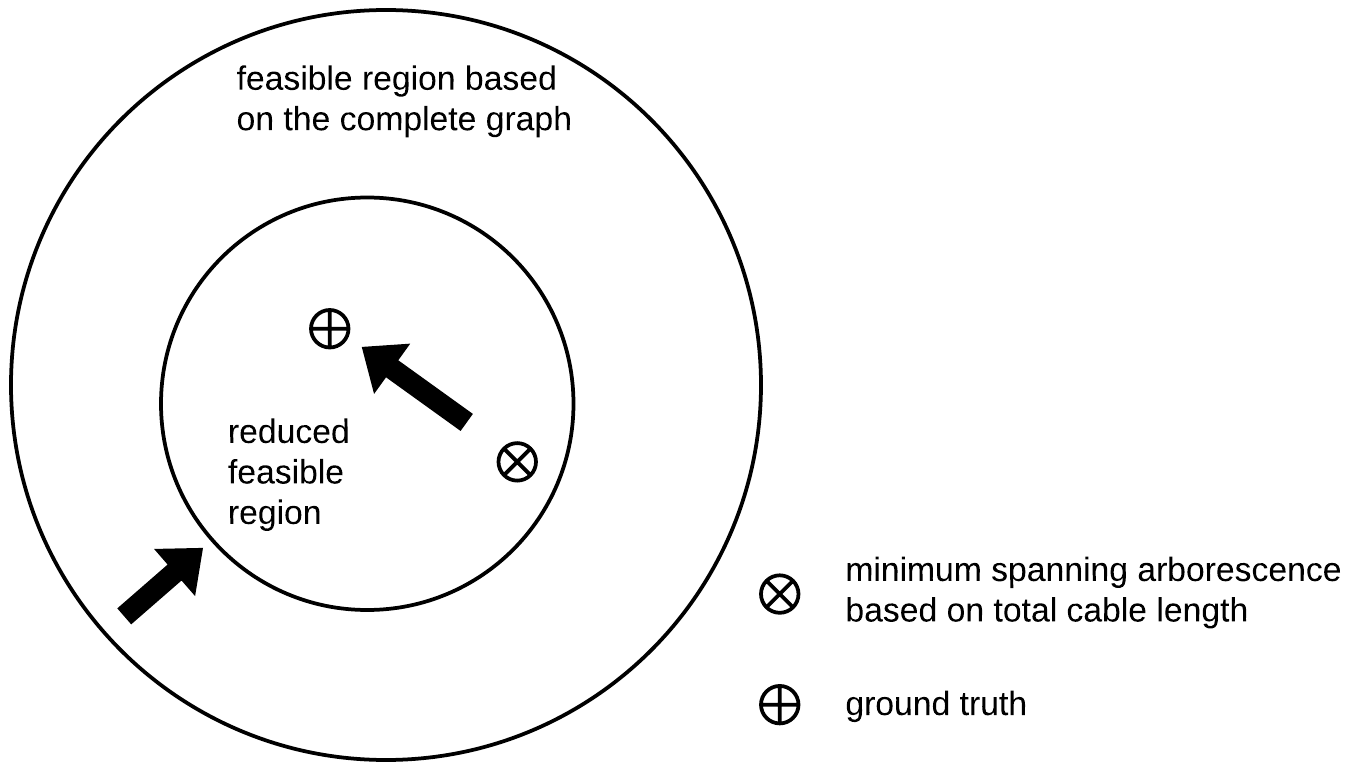
\includegraphics[width=0.7\linewidth]{Pictures/figFeasibleRegion} \end{center}

In this project, \textbf{local search heuristic algorithm} is proposed to to move
from \(\bigotimes\) to \(\bigoplus\):

\begin{table}[H]
\centering
\begin{tabular}[t]{l|l|l}
\hline
function & what it does & in this project\\
\hline
objective & assess candidate & pseudo linearised power flow\\
\hline
neighbourhood & generate candidate & rank spanning arborescence\\
\hline
\end{tabular}
\end{table}

\begin{itemize}
\tightlist
\item
  The starting point is found by minimum spanning arborescence
\item
  Every candidate is reachable from the starting point.
\item
  Ground truth should be found before long.
\item
  Not in parallel.
\end{itemize}

\hypertarget{direct-impedance-method}{%
\chapter{Direct Impedance Method}\label{direct-impedance-method}}

Discussion is based on one-line model. Can be generalised for multi-phase
model.

\begin{itemize}
\tightlist
\item
  Model RDF with one bus impedance matrix.
\item
  Calculate power flow using fixed point method.
\end{itemize}

\hypertarget{BIM}{%
\section{Bus Impedance Matrix}\label{BIM}}

Current injection to flow:
\[
  \bar{\boldsymbol{I}}_{\text{edge}} =
  - \boldsymbol{K} \bar{\boldsymbol{I}}
\]

where \textbf{edge path incidence matrix (EPI)}, \(\boldsymbol{K}\).

Voltage drop to nodal voltage:
\[
  \bar{\boldsymbol{V}} =
  \bar{\boldsymbol{V}}_{\text{zero}}
  - \boldsymbol{K}^{\top} \boldsymbol{\bar{Z}}_\text{edge}
  \bar{\boldsymbol{I}}_{\text{edge}} 
\]

where \textbf{edge impedance diagonal block matrix (EIDB)},
\(\boldsymbol{\bar{Z}}_\text{edge}\).

Alternating current power flow:
\[
  \bar{\boldsymbol{V}} = \bar{\boldsymbol{V}}_{\text{zero}}
    + \left( \boldsymbol{K}^{\top} \boldsymbol{\bar{Z}}_\text{edge}
    \boldsymbol{K} \right) \bar{\boldsymbol{I}}
\]

\begin{center}\rule{0.5\linewidth}{0.5pt}\end{center}

\textbf{Bus impedance matrix (BIM)}, \(\boldsymbol{\bar{Z}}\), is defined as:
\[ \begin{aligned}
  \boldsymbol{\bar{Z}}
    &= \boldsymbol{K}^{\top} \boldsymbol{\bar{Z}}_\text{edge}
    \boldsymbol{K} \\
    &= \boldsymbol{R} + j \boldsymbol{X}
\end{aligned} \]

where \textbf{bus resistance matrix (BRM)}, \(\boldsymbol{R}\): real part of entries
in BIM.

Five steps to build BIM:

\begin{enumerate}
\def\labelenumi{\arabic{enumi}.}
\tightlist
\item
  Define a unit impedance matrix.
\item
  Calculate edge impedance matrices for cables.
\item
  Build EIDB.
\item
  Obtain EPI based on topology.
\item
  Calculate BIM using EIDB and EPI.
\end{enumerate}

\hypertarget{fixed-point-method}{%
\section{Fixed Point Method}\label{fixed-point-method}}

To calculate power flow in one snapshot, given power injections, the following
procedure is repeated:
\[ \begin{aligned}
    \boldsymbol{\bar{I}} &= \boldsymbol{\underline{P}}
      \otimes \boldsymbol{\underline{V}}_\text{previous} \\
    \boldsymbol{\bar{V}}
    &= \boldsymbol{\bar{Z}} \boldsymbol{\bar{I}}
      + \boldsymbol{\bar{V}}_\text{zero} \\
    \epsilon
    &= \left( \boldsymbol{\bar{V}} - \boldsymbol{\bar{V}} \right)^\top
      \left( \boldsymbol{\bar{V}} - \boldsymbol{\bar{V}} \right)
\end{aligned} \]
until \(\epsilon\) is smaller than a pre-defined threshold.

\hypertarget{linearised-power-flow}{%
\chapter{Linearised Power Flow}\label{linearised-power-flow}}

Three ways to calculated BRM:

\begin{itemize}
\tightlist
\item
  Real part of entries in BIM.
\item
  \protect\hyperlink{linearVoltageDrop}{Using EPI and ERDB}.
\item
  Lowest common ancestor problem.
\end{itemize}

\hypertarget{linearVoltageDrop}{%
\section{Linearised Voltage Drop}\label{linearVoltageDrop}}

With power flow at source of edge \(k\), \(\bar{S}_{\text{source}, k}\):
\[
\bar{I}_{\text{edge}, k}
  = \frac{\underline{S}_{\text{source}, k}}{\underline{V}_i} \\
\]

Voltage drop:
\[
\begin{aligned}
  \bar{V}_{\text{edge}, k}
  &= \bar{I}_{\text{edge}, k} \bar{Z}_{\text{edge}, k} \\
  &= \frac{
    \underline{S}_{\text{source}, k} \bar{Z}_{\text{edge}, k}
  }{\underline{V}_i} \\
  &= \frac{
    \left(P_{\text{source}, k} - j Q_{\text{source}, k} \right)
    \left(R_{\text{edge}, k} + j X_{\text{edge}, k} \right)
  }{\underline{V}_i} \\
  &= \frac{
    R_{\text{edge}, k} P_{\text{source}, k}
    + X_{\text{edge}, k} Q_{\text{source}, k}
  }{\underline{V}_i}
  + j \frac{
    X_{\text{edge}, k} P_{\text{source}, k}
    - R_{\text{edge}, k} Q_{\text{source}, k}
  }{\underline{V}_i}
\end{aligned}
\]

Then:
\[
V_{\text{edge}, k} =
  \frac{R_{\text{edge}, k}}{V_\text{rate}} P_{\text{source}, k}
\]

\begin{itemize}
\tightlist
\item
  Ignore imaginary part.
\item
  Replace \(\underline{V}_i\) with \(V_\text{rate}\).
\end{itemize}

\hypertarget{linearised-voltage}{%
\section{Linearised Voltage}\label{linearised-voltage}}

Voltage drop to nodal voltage:
\[
\boldsymbol{V}
  = \boldsymbol{V}_\text{zero}
  - \frac{1}{V_\text{rate}} \boldsymbol{K}^{\top}
  \boldsymbol{R}_\text{edge} \boldsymbol{P}_\text{source}
\]

Power injection to flow:
\[
\boldsymbol{P}_\text{source}
  = \boldsymbol{K}
  \left(\boldsymbol{P} - \boldsymbol{P}_\text{loss} \right)
\]

\begin{center}\rule{0.5\linewidth}{0.5pt}\end{center}

Voltage magnitude can be calculated using BRM and real power injections:
\[ \begin{aligned}
  \boldsymbol{V} &= \boldsymbol{V}_\text{zero} + \frac{1}{V_\text{rate}}
    \left(
      \boldsymbol{K}^{\top} \boldsymbol{R}_\text{edge} \boldsymbol{K}
    \right) \boldsymbol{P} \\
  {} &= \boldsymbol{V}_\text{zero}
      + \frac{1}{V_\text{rate}} \boldsymbol{R} \boldsymbol{P}
\end{aligned} \]

\begin{itemize}
\tightlist
\item
  To \protect\hyperlink{assessment}{assess candidate} by calculating power injection using
  voltage magnitudes.
\end{itemize}

\hypertarget{BRM}{%
\section{Bus Resistance Matrix}\label{BRM}}

\begin{itemize}
\tightlist
\item
  Step-down transformer is ignored, so bus 1 is not included.
\item
  Bus 2 is the root.
\item
  There are 69 PQ buses, and there are 207 channels.
\item
  207 rows and 207 columns.
\end{itemize}

\begin{center}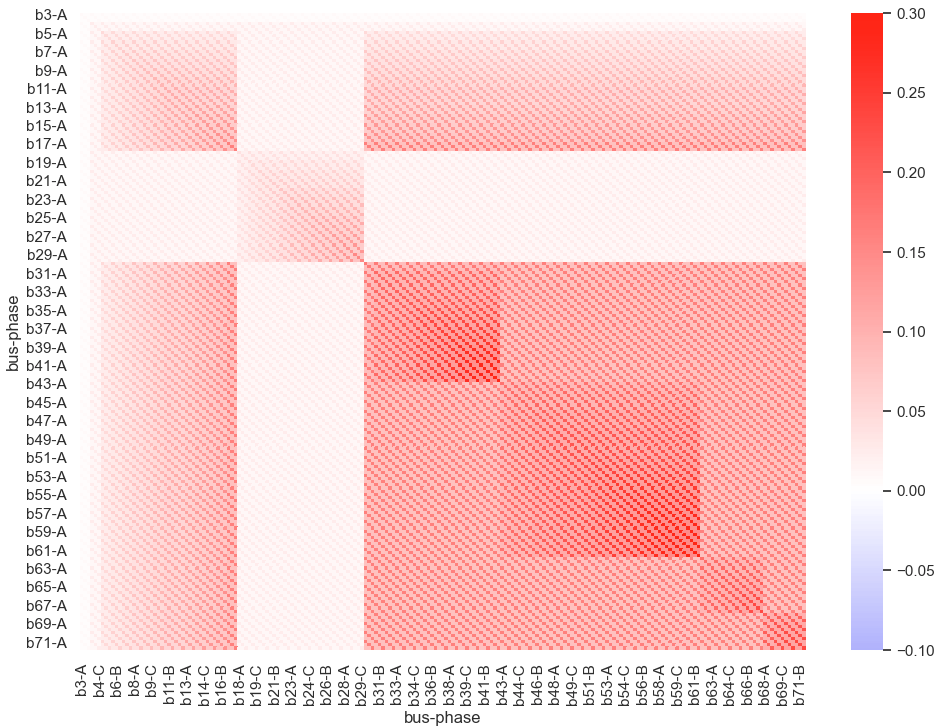
\includegraphics{Pictures/figHeatmapBRM} \end{center}

\hypertarget{LCA}{%
\subsection*{Lowest Common Ancestor Problem}\label{LCA}}
\addcontentsline{toc}{subsection}{Lowest Common Ancestor Problem}

Entry \((i, j)\) is the sum of edge resistances in the common path to the root of
bus \(i\) and \(j\). That is sum of edge resistances in the path from the root to
the lowest common ancestor (LCA) of bus \(i\) and \(j\):
\[
R_{i, j}=\sum_{k \in U_{i} \cap U_{j}} R_{\text {edge }, k}
\]
where \(U_{i}\) is set of edges on path from the root to bus \(i\).

\begin{itemize}
\tightlist
\item
  BRM can be calcualted efficiently using LCA for all pairs of buses.
\item
  The pattern can be used in future work.
\end{itemize}

For example,

\begin{center}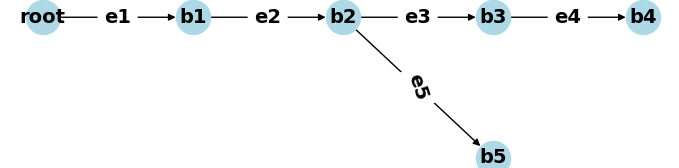
\includegraphics[width=0.7\linewidth]{Pictures/figCaseSix} \end{center}

\begin{itemize}
\tightlist
\item
  LCA of b3 and b5 is b2. Entry for b3, b5 is \(R_\text{e1} + R_\text{e2}\)
\item
  LCA of b4 and b5 is still b2. Entry for b4, b5 is still \(R_\text{e1} + R_\text{e2}\).
\end{itemize}

\hypertarget{pseudo-linearised-power-flow}{%
\section{Pseudo Linearised Power Flow}\label{pseudo-linearised-power-flow}}

Based on linearised power flow, \(\boldsymbol{V} = \boldsymbol{V}_\text{zero} + \frac{1}{V_\text{rate}} \boldsymbol{R} \boldsymbol{P}\):
\[ \begin{aligned}
    \boldsymbol{P}_\text{assess} =
    V_\text{rate} \boldsymbol{R}^{\top}
    \left( \boldsymbol{V} - \boldsymbol{V}_\text{zero} \right)
\end{aligned} \]
which is referred to as \textbf{pseudo linearised power flow}.

The inversed BRM for case-70 looks like:

\begin{center}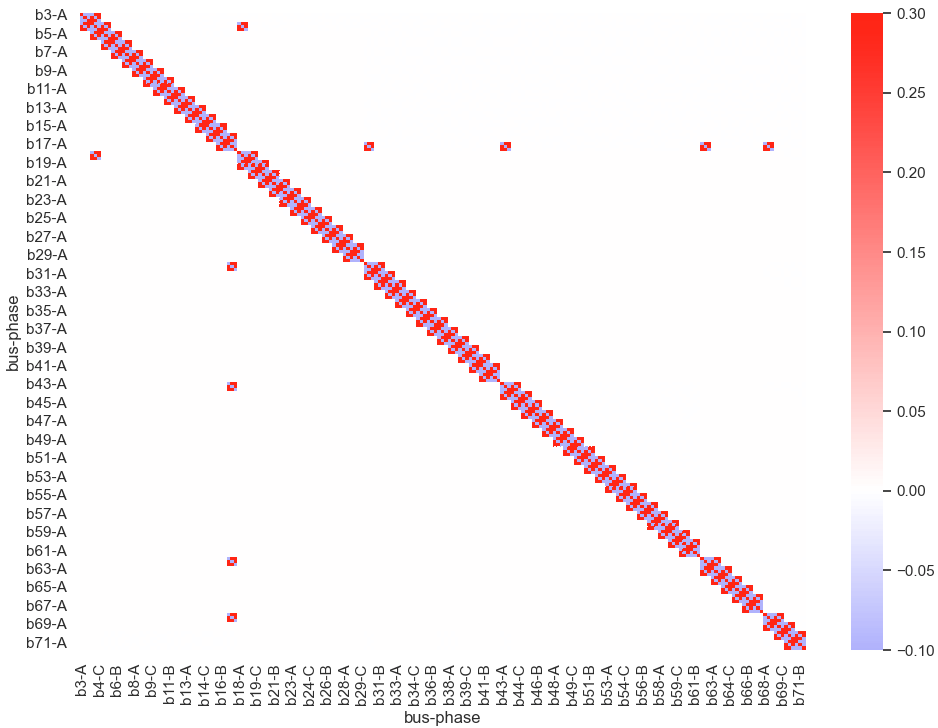
\includegraphics{Pictures/figHeatmapBrmInv} \end{center}

\begin{itemize}
\tightlist
\item
  Voltage magnitude at any channel can have a huge impact.
\item
  The pattern can be used in future work.
\end{itemize}

\hypertarget{assessment}{%
\section{Assessment of Candidate}\label{assessment}}

The second term in the objective function is:
\[ \begin{aligned}
  \mathcal{H}(\boldsymbol{R}) =
  \left[
    (\boldsymbol{P}_\text{assess} - \boldsymbol{P})
    \otimes \boldsymbol{O}
  \right]^\top
  \cdot \left[
    (\boldsymbol{P}_\text{assess} - \boldsymbol{P})
    \otimes \boldsymbol{O}
  \right]
  / |\mathcal{O}|
\end{aligned} \]
where:

\begin{itemize}
\tightlist
\item
  \(\mathcal{O}\): set of observed active channels
\item
  \(\boldsymbol{O}\): binary vector indicating observed active channels
\item
  Entries for unobserved active channel are ignored.
\end{itemize}

\hypertarget{error-from-linearisation}{%
\subsection*{Error from Linearisation}\label{error-from-linearisation}}
\addcontentsline{toc}{subsection}{Error from Linearisation}

Box plot for assessment results of case-70 with respect to different number of
observed active channels, based on ground truth and 50 snapshots\footnote{during
  00:00:00 and 00:00:50 on Dec 2, 2020 from Sonnen data set.}.

\begin{center}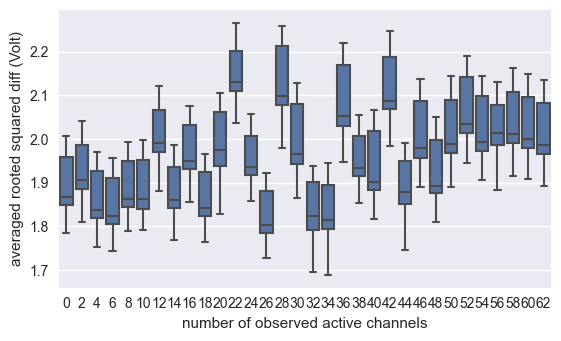
\includegraphics{Pictures/figErrorObsBRM} \end{center}

\begin{itemize}
\tightlist
\item
  Error is aleady reduced to 1.7 \textasciitilde{} 2.2.
\item
  Rated voltage magnitudes will increase the error dramatically.
\item
  Full observability over voltage magnitudes for now.
\end{itemize}

\hypertarget{VSM}{%
\section{Voltage Sensitivity Matrix}\label{VSM}}

\hypertarget{result-and-discussion}{%
\chapter{Result and Discussion}\label{result-and-discussion}}

\hypertarget{result-for-case-70}{%
\section{Result for Case-70}\label{result-for-case-70}}

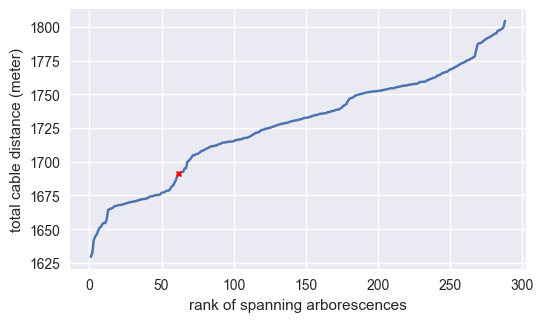
\includegraphics{Pictures/distances_288.png}

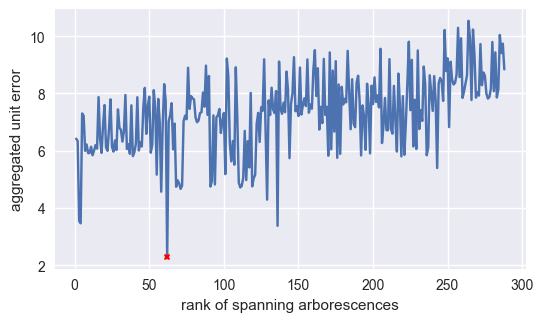
\includegraphics{Pictures/errors_288.png}

\hypertarget{project-flowchart}{%
\section{Project Flowchart}\label{project-flowchart}}

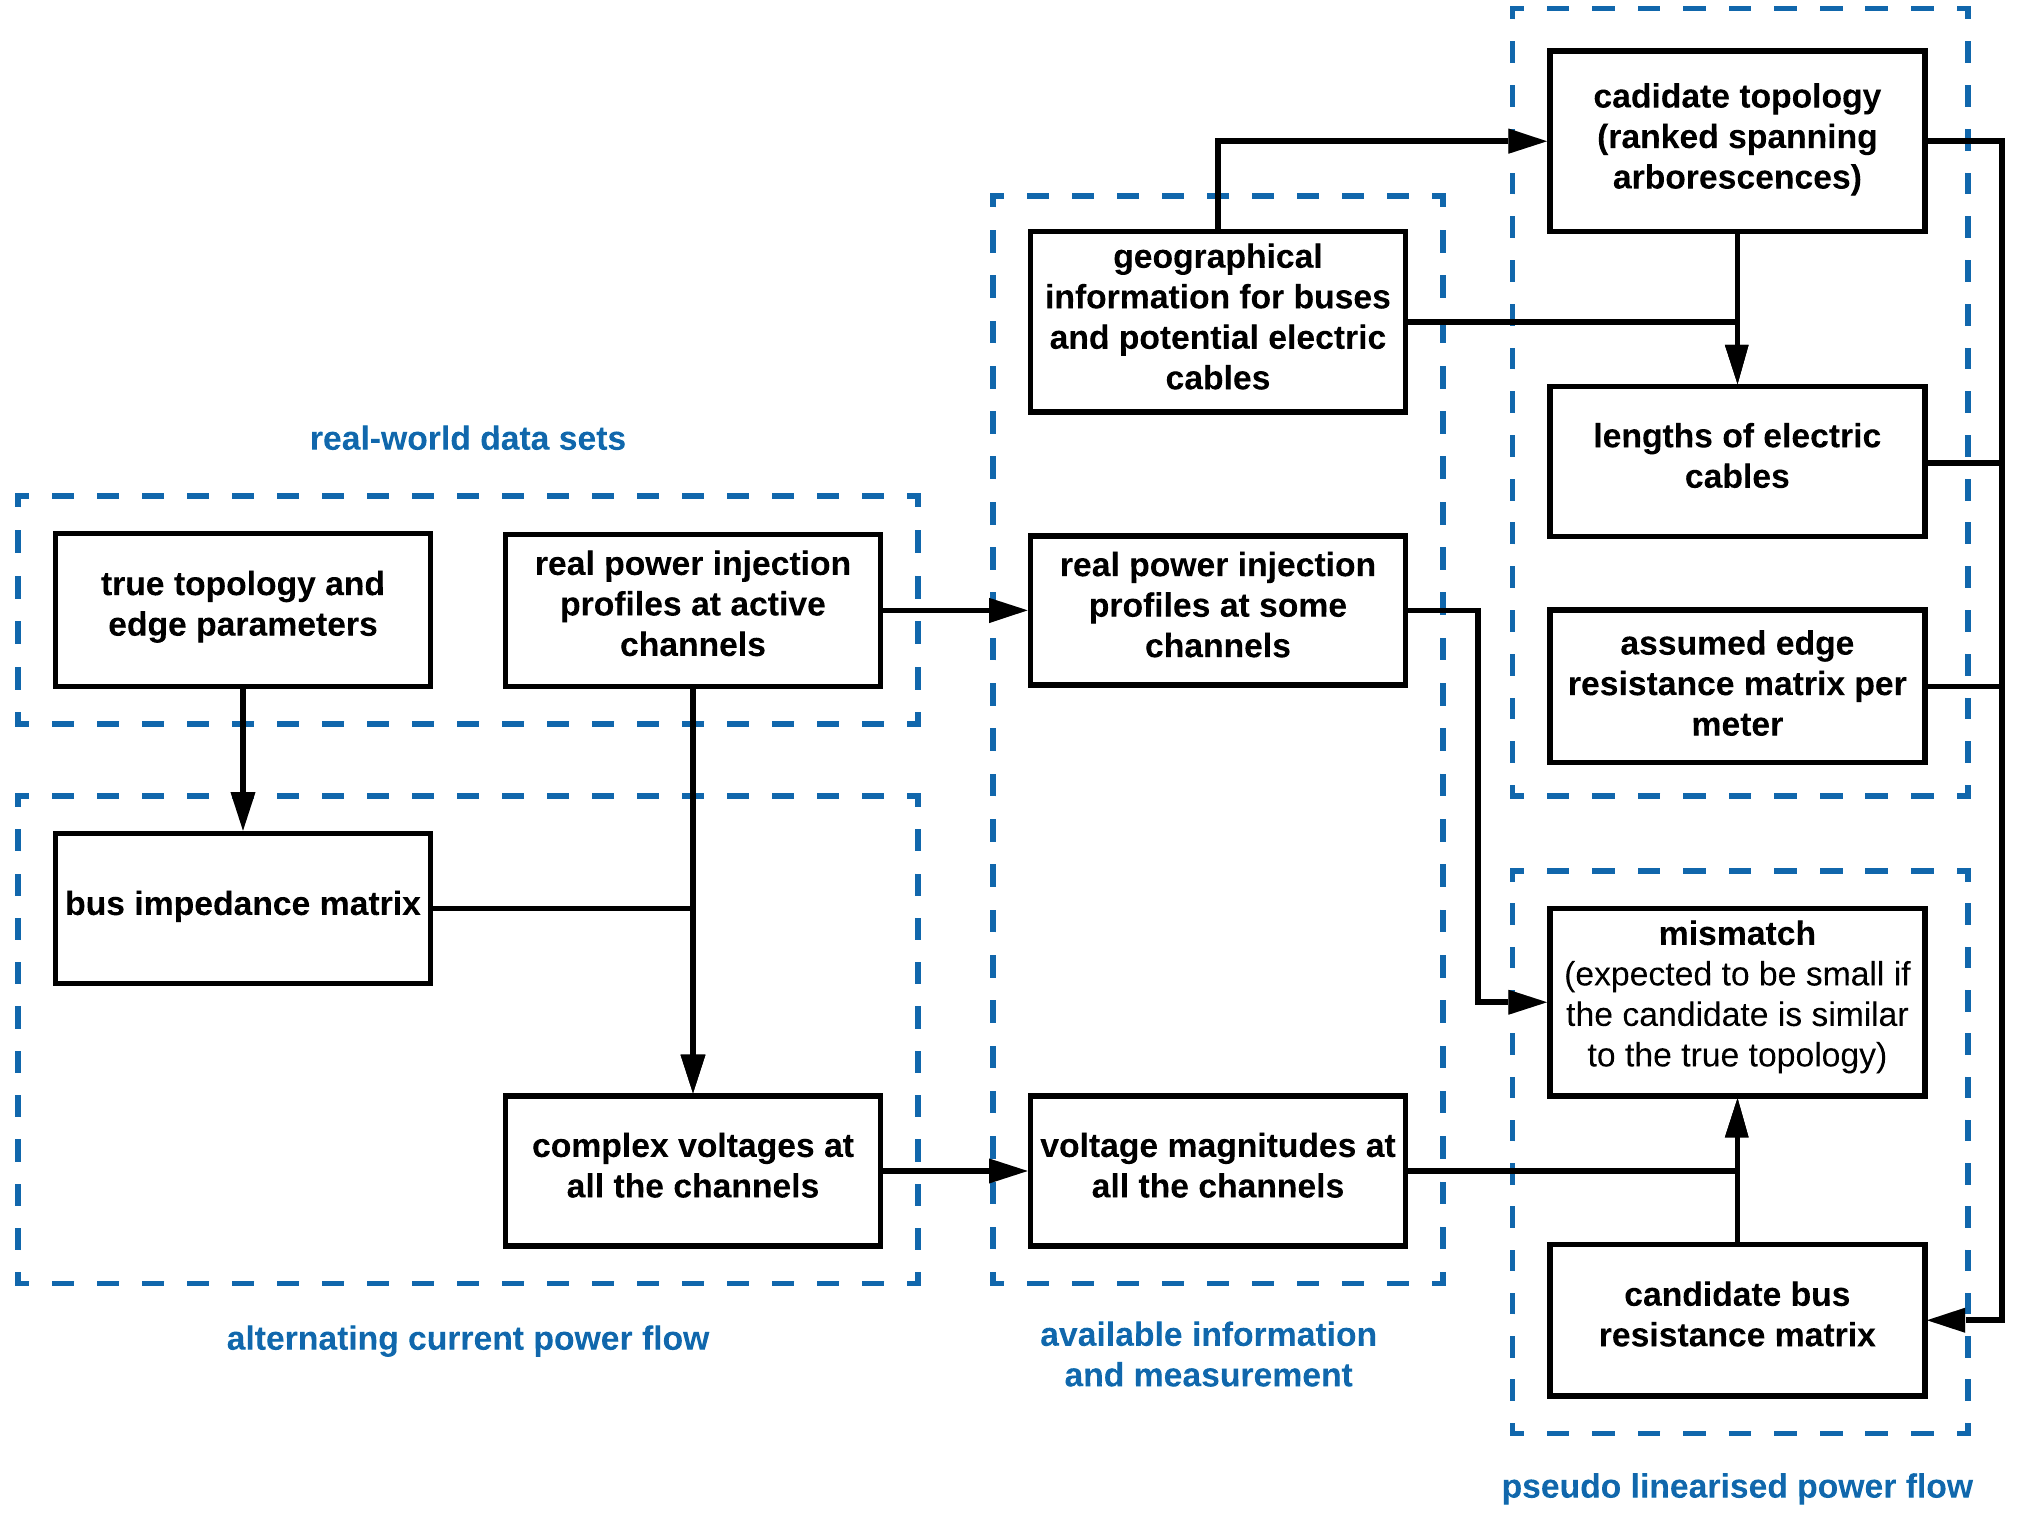
\includegraphics{Pictures/figFlowchartRotate.png}

\hypertarget{summary}{%
\section{Summary}\label{summary}}

All in all, there are four steps in the proposed framework for topology inference:

\begin{enumerate}
\def\labelenumi{\arabic{enumi}.}
\tightlist
\item
  Shrink feasible region (reduce the number of SAs) by removing overlapping
  edges.
\item
  Measure the size of feasible region by counting number of SAs.
\item
  Get candidates sequentially by ranking SAs according to total cable lengths.
\item
  Assess candidates based on available measurements.
\end{enumerate}

\hypertarget{issues}{%
\subsection*{Issues}\label{issues}}
\addcontentsline{toc}{subsection}{Issues}

\begin{enumerate}
\def\labelenumi{\arabic{enumi}.}
\tightlist
\item
  Too many spanning arborescences. (\protect\hyperlink{overlapping}{remove overlapping edges})
\item
  Full observability over voltage magnitudes. (\protect\hyperlink{BRM}{matrices with full
  rank})
\item
  Error in linearised power flow calculation. (\protect\hyperlink{VSM}{voltage sensitivity
  matrix})
\end{enumerate}

\hypertarget{future-work}{%
\subsection*{Future Work}\label{future-work}}
\addcontentsline{toc}{subsection}{Future Work}

\begin{itemize}
\tightlist
\item
  How to detect more impossible potential edges. (for issue 1)
\item
  How to assess candidates based on a fraction. (for issue 2)
\item
  How to use voltage sensitivity matrix in linearised power flow. (for issue 3)
\end{itemize}

  \bibliography{bibliography.bib}

\end{document}
